\documentclass[10pt]{article}
\usepackage[ngerman]{babel}
\usepackage[utf8]{inputenc}
\usepackage[T1]{fontenc}
\usepackage{amsmath}
\usepackage{amsfonts}
\usepackage{amssymb}
\usepackage[version=4]{mhchem}
\usepackage{stmaryrd}
\usepackage{graphicx}
\usepackage[export]{adjustbox}
\graphicspath{ {./images/} }

\title{Hauptprüfung Abiturprüfung 2021 - Leistungsfach }

\author{Alexander Schwarz\\
www.mathe-aufgaben.com}
\date{}


\begin{document}
\maketitle
 Baden-Württemberg\section*{Pflichtteil - Aufgabensatz 2 \\
 Hilfsmittel: keine allgemeinbildende Gymnasien }
August 2021

\section*{Aufgabe 1: (0,5 VP und 2 VP)}
Gegeben ist die Funktion $f$ mit $f(x)=4 x-x^{2}$. Die Abbildung zeigt ihren Graphen $G_{f}$ sowie die Tangenten an $G_{f}$ in den Schnittpunkten mit der x-Achse.\\
a) Weisen Sie nach: Die Tangente an $G_{f}$ an der Stelle $\mathrm{x}=0$ hat die Steigung 4.\\
b) Die beiden Tangenten schneiden sich in einem Punkt S. Berechnen Sie den\\
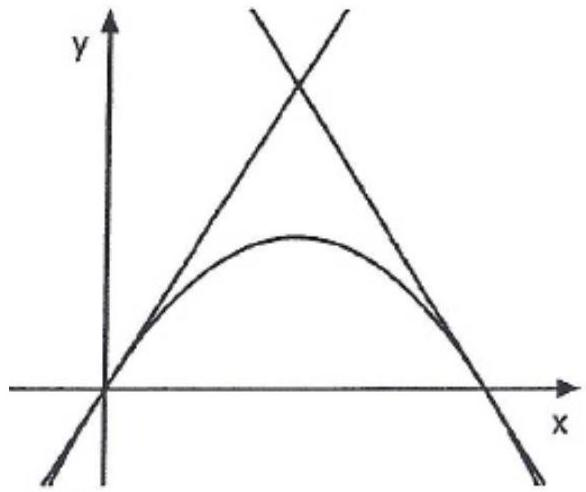
\includegraphics[max width=\textwidth]{2025_04_24_b94e5afb4f169f5c07a3g-2(1)} Abstand des Punktes $S$ vom Ursprung.

\section*{Aufgabe 2: (2,5 VP)}
Die Abbildung zeigt die Graphen der Funktionen $f$ und $g$ mit $f(x)=e^{-x}$ und $g(x)=x+1$, deren Schnittpunkt auf der $y$-Achse liegt.

Die Graphen begrenzen mit der x-Achse und der Geraden $x=u(u>0)$ eine Fläche.\\
Diese Fläche wird von der y-Achse in zwei inhaltsgleiche Teilflächen geteilt. Berechnen Sie den Wert von u.\\
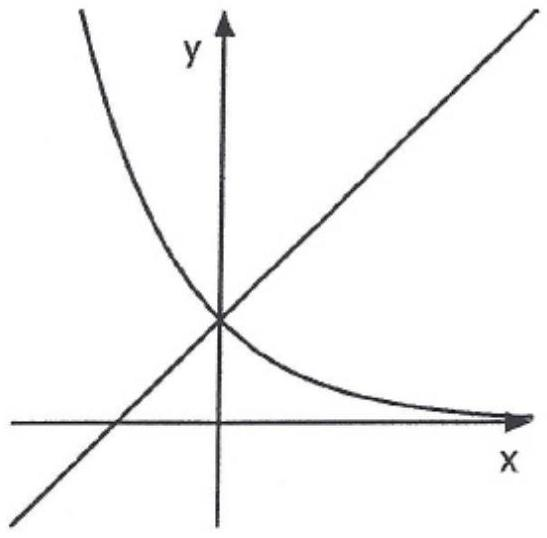
\includegraphics[max width=\textwidth, center]{2025_04_24_b94e5afb4f169f5c07a3g-2}

\section*{Aufgabe 3: (2,5 VP)}
Die Abbildung zeigt den Graphen einer trigonometrischen Funktion. Bestimmen Sie einen möglichen Funktionsterm.\\
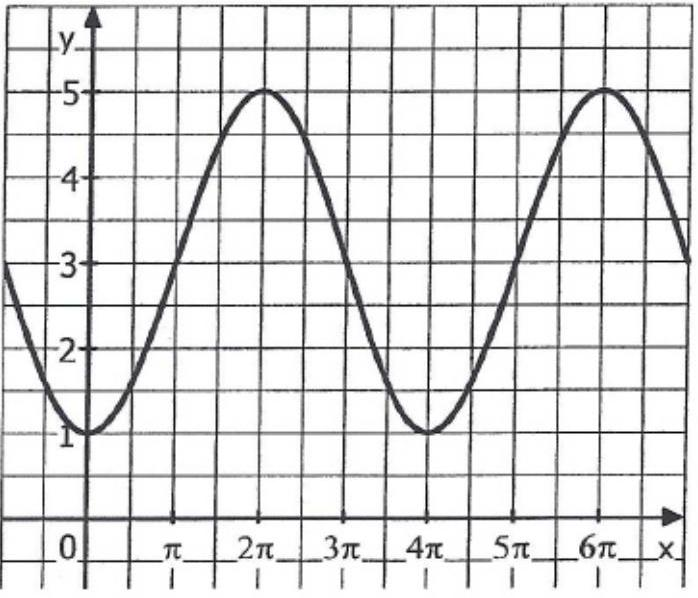
\includegraphics[max width=\textwidth, center]{2025_04_24_b94e5afb4f169f5c07a3g-2(2)}

\section*{Aufgabe 4: (1 VP und 1,5 VP)}
Die Abbildung zeigt den Graphen der Funktion f.\\
a) Begründen Sie, dass die Ableitungsfunktion $\mathrm{f}^{\prime}$ im Intervall [5;8] nicht monoton ist.\\
b) Bestimmen Sie die Anzahl der Nullstellen der Funktion $\mathrm{I}_{2}$ mit $\mathrm{I}_{2}(\mathrm{x})=\int_{2}^{\mathrm{x}} \mathrm{f}(\mathrm{t}) \mathrm{dt}$,\\
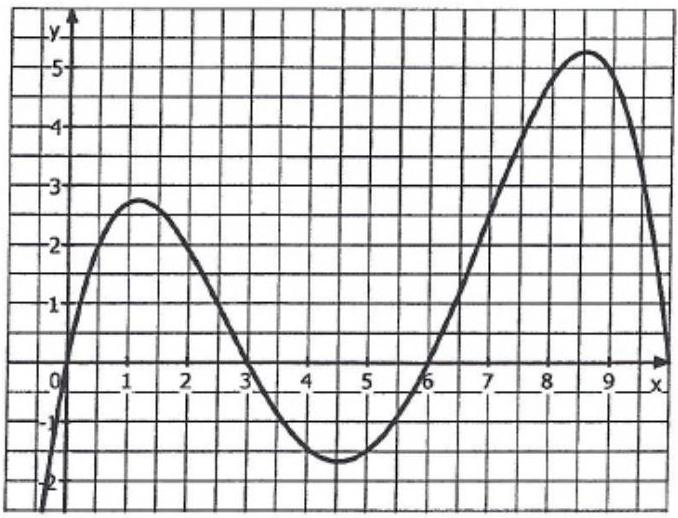
\includegraphics[max width=\textwidth]{2025_04_24_b94e5afb4f169f5c07a3g-3} $2 \leq x \leq 9$

\section*{Aufgabe 5: (1,5 VP und 1 VP)}
Gegeben sind die Punkte $A(6|4|-1)$ und $B(0|-5| 2)$ sowie die Ebene E: $2 x_{1}-2 x_{2}+x_{3}=6$.\\
a) Die Gerade durch $A$ und $B$ schneidet $E$ im Punkt $S$.

Bestimmen Sie die Koordinaten von S .\\
b) Untersuchen Sie, ob der Punkt S auf der Strecke AB liegt.

\section*{Aufgabe 6: (0,5 VP und 2 VP)}
Gegeben ist die Ebene $\mathrm{E}: 3 \mathrm{x}_{2}-4 \mathrm{x}_{3}=2$.\\
a) Beschreiben Sie die besondere Lage von E im Koordinatensystem.\\
b) Die Ebene F ist orthogonal zu E und hat zur $\mathrm{x}_{1}$-Achse den Abstand 2.

Bestimmen Sie eine mögliche Koordinatengleichung von F.

\section*{Aufgabe 7: (1 VP und 1,5 VP)}
Ein Verein erhält eine Lieferung gebrauchter Computer und Bildschirme. Von den 10 Computern und 15 Bildschirmen funktionieren jeweils drei Geräte nicht. Jemand wählt zufällig einen Computer und einen Bildschirm aus.\\
a) Berechnen Sie die Wahrscheinlichkeit dafür, dass beide ausgewählten Geräte funktionieren.\\
b) Nach Inbetriebnahme der zwei ausgewählten Geräte stellt sich heraus, dass beide Geräte funktionieren. Anschließend wählt jemand aus den übrigen Geräten der Lieferung zwei Computer aus. Berechnen Sie die Wahrscheinlichkeit dafür, dass mindestens einer der beiden zuletzt ausgewählten Computer funktioniert.

\section*{Aufgabe 8: (0,5 VP und 2 VP)}
Ein idealer Würfel wird 20-mal geworfen. Betrachtet wird die Anzahl der gewürfelten Sechsen.\\
Gegeben sind drei Terme:\\
I: $\left(\frac{1}{6}\right)^{11} \cdot\left(\frac{5}{6}\right)^{9}$\\
II: $\binom{20}{11} \cdot\left(\frac{1}{6}\right)^{11} \cdot\left(\frac{5}{6}\right)^{9}$\\
III: $1-\binom{20}{9} \cdot\left(\frac{5}{6}\right)^{9} \cdot\left(\frac{1}{6}\right)^{11}$\\
a) Geben Sie an, mit welchem der drei Terme die Wahrscheinlichkeit des Ereignisses „Es wird genau 11-mal eine Sechs gewürfelt." berechnet werden kann.\\
b) Formulieren Sie für jeden der beiden verbleibenden Terme ein Ereignis im Sachzusammenhang, dessen Wahrscheinlichkeit mit dem jeweiligen Term berechnet werden kann.

\section*{Lösungen}
\section*{Aufgabe 1:}
a) $f(x)=4 x-x^{2}$\\
$f^{\prime}(x)=4-2 x$\\
Steigung an der Stelle $x=0: f^{\prime}(0)=4$\\
Damit ist der Nachweis erbracht.\\
b) Die Tangente g im Ursprung besitzt die Gleichung $\mathrm{y}=4 \mathrm{x}$ (Steigung gemäß a)).

Der x-Wert des Schnittpunktes S entspricht aus Symmetriegründen dem x-Wert des Hochpunktes der Parabel.\\
Berechnung der Extremstelle der Parabel: $f^{\prime}(x)=0$\\
$4-2 x=0 \Leftrightarrow x=2$\\
Einsetzen von $\mathrm{x}=2$ in die Tangente g ergibt $\mathrm{y}=8$.\\
Koordinaten von S: S(2|8).\\
Abstand von S zum Ursprung mit dem Satz des Pythagoras: $\overline{\mathrm{OS}}=\sqrt{2^{2}+8^{2}}=\sqrt{68}$

\section*{Aufgabe 2:}
Skizze:
\begin{center}
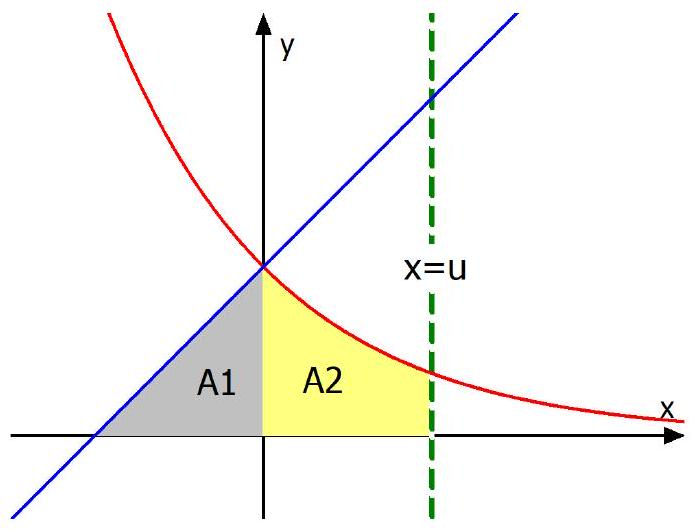
\includegraphics[max width=\textwidth]{2025_04_24_b94e5afb4f169f5c07a3g-5}
\end{center}

Schnittpunkt der Gerade g mit der x-Achse: A(-1|0)\\
Schnittpunkt der Gerade g mit der y-Achse: $\mathrm{P}(0 \mid 1$\\
$\mathrm{A} 1=\mathrm{A}_{\text {Dreieck }}=\frac{1}{2} \cdot 1 \cdot 1=\frac{1}{2}$\\
$\mathrm{A} 2=\int_{0}^{u} \mathrm{e}^{-\mathrm{x}} \mathrm{dx}=\left[-\mathrm{e}^{-\mathrm{x}}\right]_{0}^{u}=-\mathrm{e}^{-\mathrm{u}}-(-1)=-\mathrm{e}^{-u}+1$\\
Bedingung: $-\mathrm{e}^{-\mathrm{u}}+1=\frac{1}{2} \Leftrightarrow \mathrm{e}^{-\mathrm{u}}=\frac{1}{2} \Leftrightarrow \mathrm{u}=-\ln \frac{1}{2}$ oder $\mathrm{u}=\ln (2)$

\section*{Aufgabe 3:}
Allgemeiner Ansatz für den Funktionsterm:\\
$f(x)=a \cdot \sin (b \cdot(x-c))+d \operatorname{oder} g(x)=a \cdot \cos (b \cdot(x-c))+d$\\
Es gilt $\mathrm{d}=\frac{\mathrm{y}_{\text {max }}+\mathrm{y}_{\text {min }}}{2}=\frac{5+1}{2}=3$.\\
Die Amplitude ist $|a|=\frac{y_{\text {max }}-y_{\text {min }}}{2}=\frac{5-1}{2}=2$.\\
Die Periode der Funktion ist $p=4 \pi$. Daraus folgt $b=\frac{2 \pi}{4 \pi}=0,5$.\\
Für die Modellierung der Funktion gibt es mehrere Möglichkeiten.\\
Modellierung als Sinusfunktion:\\
Die Wendestelle mit positiver Steigung befindet sich bei $\mathrm{x}=\pi$.\\
Somit ist $\mathrm{c}=\pi$\\
Ergebnis: $f(x)=2 \cdot \sin (0,5 \cdot(x-\pi))+3$\\
Modellierung als Kosinusfunktion:\\
Der Hochpunkt befindet sich bei $x=2 \pi$.\\
Somit ist $c=2 \pi$\\
Ergebnis: $f(x)=2 \cdot \cos (0,5 \cdot(x-2 \pi))+3$\\
Modellierung als an der x-Achse gespiegelte Kosinusfunktion:\\
Da der Tiefpunkt auf der y -Achse liegt, ist $\mathrm{c}=0$\\
Ergebnis: $f(x)=-2 \cdot \cos (0,5 \cdot x)+3$

\section*{Aufgabe 4:}
a) Die Ableitungsfunktion $f^{\prime}$ wäre dann monoton, wenn im Intervall $[5 ; 8] f^{\prime \prime}(x) \geq 0$ oder $f^{\prime \prime}(x) \leq 0$ ist.\\
An der Stelle $x=5$ ist das Schaubild von $f$ linksgekrümmt, also gilt $f^{\prime \prime}(5)>0$.\\
An der Stelle $x=8$ ist das Schaubild von $f$ rechtsgekrümmt, also gilt $f^{\prime \prime}(8)<0$.\\
b)
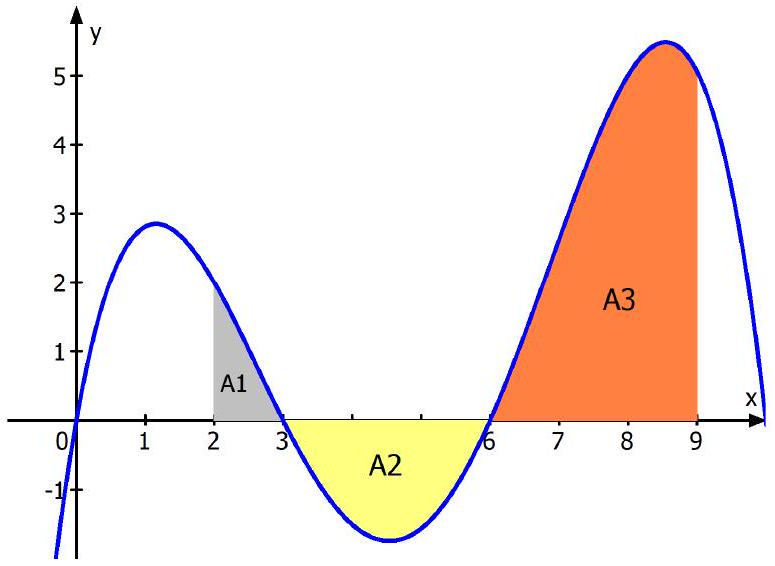
\includegraphics[max width=\textwidth, center]{2025_04_24_b94e5afb4f169f5c07a3g-7}

Die Integralfunktion besitzt die Nullstelle $x=2$, da $I_{2}(2)=\int_{2}^{2} f(t) d t=0$\\
Durch Abzählen der Kästchen ergibt sich etwa $A 1 \approx 1$ und $A 2 \approx 3,5$ und $A 3 \approx 10,5$.

Somit gibt es eine Stelle $x^{*}$ im Intervall [3;6] mit $I_{2}\left(x^{*}\right)=\int_{2}^{x^{*}} f(t) d t=0$\\
Es gilt $\mathrm{I}_{2}(6)=\int_{2}^{6} f(\mathrm{t}) \mathrm{dt} \approx 1-3,5=-2,5$.\\
Da $A 3 \approx 10,5$ ist, gibt es eine Stelle $x^{* *}$ im Intervall [6;9] mit $I_{2}\left(x^{* *}\right)=\int_{2}^{x^{* *}} f(t) d t=0$ ist.\\[0pt]
Insgesamt besitzt die Integralfunktion 3 Nullstellen im Intervall [2;9].

\section*{Aufgabe 5:}
a) Gleichung der Gerade durch $A$ und $B: g: \vec{x}=\left(\begin{array}{c}6 \\ 4 \\ -1\end{array}\right)+t \cdot\left(\begin{array}{c}-6 \\ -9 \\ 3\end{array}\right)$

Schnittpunkt von g und E:

$$
\begin{aligned}
& 2(6-6 t)-2(4-9 t)+(-1+3 t)=6 \\
& \Leftrightarrow 12-12 t-8+18 t-1+3 t=6 \\
& \Leftrightarrow 9 t=3 \Leftrightarrow t=\frac{1}{3}
\end{aligned}
$$

Einsetzen des t-Wertes in g ergibt den Schnittpunkt $S(4|1| 0)$\\
b) Da der Parameterwert $\mathrm{t}=\frac{1}{3}$ aus Teilaufgabe a) im Intervall $(0 ; 1)$ liegt, befindet sich der Punkt S zwischen den Punkten A und B (also auf der Strecke $A B)$.

\section*{Aufgabe 6:}
a) Da die $\mathrm{x}_{1}$-Koordinaten des Normalenvektors der Ebene Null ist, ist die Ebene E parallel zur $\mathrm{x}_{1}$-Achse.\\
b) Der Normalenvektor der Ebene E ist ein Spannvektor von F.

Da die Ebene F parallel zur $\mathrm{x}_{1}$-Achse ist, besitzt sie außerdem den Spannvektor $\overrightarrow{\mathrm{u}}=\left(\begin{array}{l}1 \\ 0 \\ 0\end{array}\right)$.\\
Normalenvektor von F: $\overrightarrow{\mathrm{n}}=\left(\begin{array}{c}0 \\ 3 \\ -4\end{array}\right) \times\left(\begin{array}{l}1 \\ 0 \\ 0\end{array}\right)=\left(\begin{array}{c}0 \\ -4 \\ -3\end{array}\right)$ bzw. $\overrightarrow{\mathrm{n}}^{*}=\left(\begin{array}{l}0 \\ 4 \\ 3\end{array}\right)$\\
Ansatz für die Koordinatengleichung: $4 \mathrm{x}_{2}+3 \mathrm{x}_{3}=\mathrm{d}$

Der Wert von d muss nun so bestimmt werden, dass ein Punkt von der $\mathrm{x}_{1}$-Achse (z.B. der Ursprung O(0|0|0) den Abstand 2 von der Ebene F besitzt.

HNF von $\mathrm{F}: \frac{4 \mathrm{x}_{2}+3 \mathrm{x}_{3}-\mathrm{d}}{5}=0$\\
$d(O, F)=\frac{|-\mathrm{d}|}{5}=2$\\
Daraus folgt $\mathrm{d}=10$ oder $\mathrm{d}=-10$\\
Mögliche Koordinatengleichung von F: $4 \mathrm{x}_{2}+3 \mathrm{x}_{3}=10$\\
Weitere mögliche Koordinatengleichung von F: $4 \mathrm{x}_{2}+3 \mathrm{x}_{3}=-10$

\section*{Aufgabe 7:}
a) $\mathrm{P}($ Computer funktioniert $)=\frac{7}{10}$\\
$P($ Bildschirm funktioniert $)=\frac{12}{15}=\frac{4}{5}$\\
$P($ beide Geräte funktionieren $)=\frac{7}{10} \cdot \frac{4}{5}=\frac{28}{50}=\frac{14}{25}$\\
b) Nach der Entnahme eines funktionierenden Computers sind von 9 Computern noch drei defekt und sechs funktionieren.

P (mindestens ein Computer funktioniert) $=1-\mathrm{P}$ (kein Computer funktioniert)

$$
=1-\frac{3}{9} \cdot \frac{2}{8}=1-\frac{1}{12}=\frac{11}{12}
$$

\section*{Aufgabe 8:}
a) Die Wahrscheinlichkeit wird mit Hilfe der Formel von Bernoulli berechnet.

Diese entspricht der Formel II.\\
b) Formel I:\\
"In den ersten 11 Würfen wird eine Sechs gewürfelt, in den nächsten 9 Würfen wird keine 6 gewürfelt."

Formel III:\\
"Es wird nicht genau 11-mal eine Sechs gewürfelt."\\
Oder:\\
Es wird nicht genau 9-mal keine Sechs gewürfelt."


\end{document}